\documentclass{llncs}

%\usepackage{makeidx}  % allows for indexgeneration
\usepackage{graphicx}

\begin{document}

\title{SWAML, from Mailing Lists to the Semantic Web}

\titlerunning{SWAML, from Mailing Lists to the Semantic Web}


\author{
Sergio Fern\'andez \and Diego Berrueta \and Jose E. Labra
}

\authorrunning{Sergio Fern\'andez et al.}

\tocauthor{Sergio Fern\'andez, Diego Berrueta, Jose E. Labra (Universidad de Oviedo)} 

\institute{Universidad de Oviedo, \\
Technical School of Computer Science, \\
Oviedo, Asturias, Spain,\\
\email{sergio@wikier.org, diego@berrueta.net, labra@uniovi.es},\\
WWW home page: \texttt{http://swaml.berlios.de/}
}

\date{1 February 2007}

\maketitle

\begin{abstract}

Mailing list archives (i.e., the messages posted up-to-now) are often published 
on the web and indexed by conventional search engines. They store a vast 
knowledge capital. However, the ability to auto-matically recognize and process 
the information is mostly lost at publishing time. As a result, the current 
mailing list archives are hard to query and have a limited use. This paper 
describes how SWAML uses Semantic Web technologies in order to avoid the
information loss and to allow new applications able to exploit this 
information in a more convenient way.

\end{abstract}

\section{Introduction}

\cite{Luke2004}

\subsection{SIOC}

SIOC (Semantically-Interlinked Online Communities) provides methods for 
interconnecting discussion methods such as blogs, forums and mailing lists 
to each other. It consists of the SIOC ontology, an open-standard machine 
readable format for expressing the information contained both explicitly 
and implicitly in internet discussion methods, of SIOC metadata producers 
for a number of popular blogging platforms and content management systems, 
and of storage and browsing/searching systems for leveraging this SIOC 
data. \cite{Breslin2005}

The goal of SIOC \footnote{\url{http://sioc-project.org/}} is to interconnect
these online communities. Community sites can include many discussion primitives,
such as bulletin boards, weblogs and mailing lists, which it have grouped under 
the concept of forum.

\begin{figure}[ht]
 \centering
 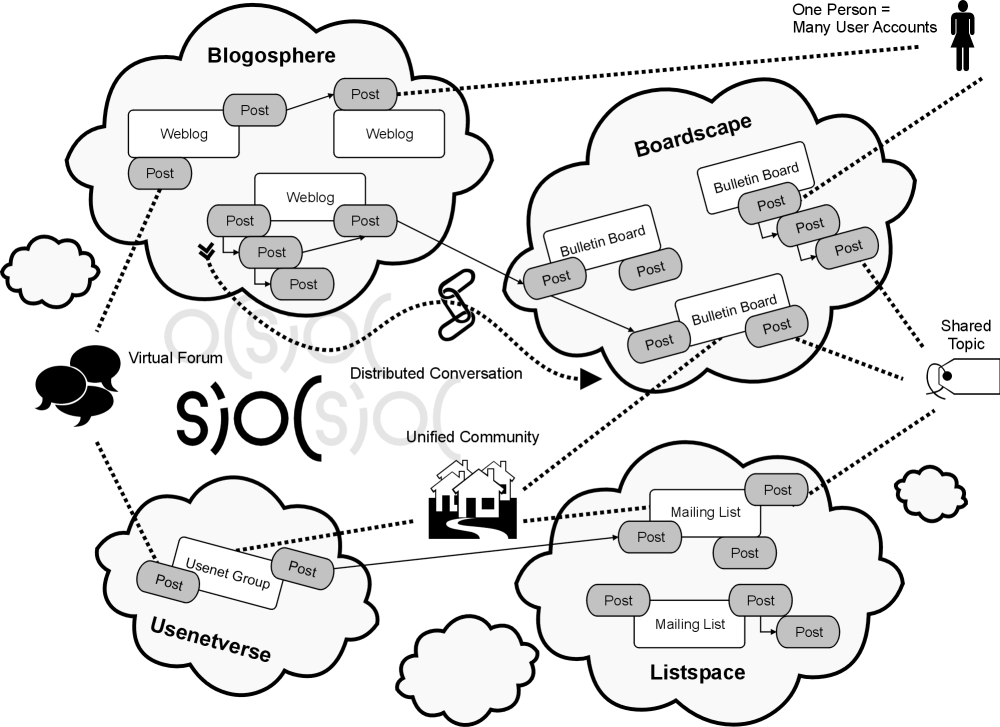
\includegraphics[bb=0 0 240 174]{images/sioc-discussion.png}
 \caption{Connections between discussion clouds with SIOC}
\end{figure}

Then \texttt{Forum} class is the most important for us at SIOC ontology. In the 
domain of a forum there are another classes at the ontology, mainly we need two
of it: \texttt{Post} and \texttt{User} 

The SIOC community has developed several wrappers that allows to export instances
of community site concepts (such as blogs o forums) in RDF format. But the effort 
is only centered in providing mappings from web-based systems, forgetting all the 
knowledgement stored in a large number of legacy systems preceding the current Web.

\section{Formal model}

FIXME (talk with Polo)

\section{Components}

In the SWAML project are involved several components, mainly three:

\begin{itemize}
 \item SWAML, the core process that exports a mailing list in RDF.
 \item Buxon, a browser for SIOC Forum instances.
 \item SWAML Ontology.
\end{itemize}


\subsection{SWAML}

FIXME

\subsection{Buxon}

FIXME

\subsection{SWAML Ontology}

Until SIOC ontology contemplates some subclasses of Forum, it's necessary 
to add some properties. Concretely in version 0.2 of our ontology 
\footnote{http://swaml.berlios.de/ns/0.2} we have reduced these properties 
to only two:

\begin{itemize}
  \item \texttt{previousByDate} to link with the previous post sent in the 
	mailing list..
  \item \texttt{nextByDate} to link with the post that was sent after by date 
	in the mailing list.
\end{itemize}

Both under the domain and the range of \texttt{sioc:Post}. Perhaps these 
properties has a minor importance to describe generic forums instances, 
but its meaning receives greater importance in the concrete scope of a 
mailing list.

\section{Conclussions and Future Work}

FIXME, interesting stuff here...

\begin{itemize}
  \item To make agile the obtaining of several mailboxes:
	To improve the experiment done using LibGmail
	
	the simplest form to obtain a lot of mail lists is to serializar to mboxes 
	the posts stored by the users in its mail accounts. The preliminar experiment 
	was made across a GMail account subscribed to a semantic web related mailing list
	\footnote{\url{http://www.johnbreslin.com/blog/2006/11/08/buxon-visor-for-siocforum-browsing/}},
	but 
\end{itemize}



\bibliographystyle{abbrv}
\bibliography{../references}
%
\end{document}
